\begin{flushleft}
\doublespacing
\subsection{Brugertest}

I TC01 testes der ud fra brugerens synsvinkel for at se, om der kommer forskellige valgmuligheder op på skærmen, der giver brugeren mulighed for at vælge, hvordan spilleren vil prøve at undslippe fængslet (se Figure \ref{Testcase01}). Det endelige resultat af GUIen kan ses i bilagene (se bilag \ref{TC01Bilag}.

\begin{figure}[H] %brug begin{figure} til alle figurer.
    \centering
    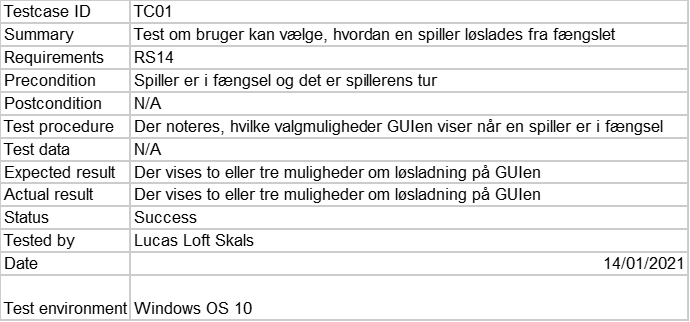
\includegraphics[width=14cm]{Report/figures/Usertests/TC01.png}
    \caption{Tabel over TC01}
    \label{Testcase01}
\end{figure}

I TC02 testes der for om spillerne kan vælge, hvilken spiller der starter ved at indtaste et heltal i en tekstboks (Se Figure \ref{Testcase02}. Når et heltal er indtastet bør en succesful test vise, at den indtastede spiller starter sin tur. Det endelige resultat af GUIen kan ses i bilagene (se bilag \ref{TC02Bilag}).

\begin{figure}[H] %brug begin{figure} til alle figurer.
    \centering
    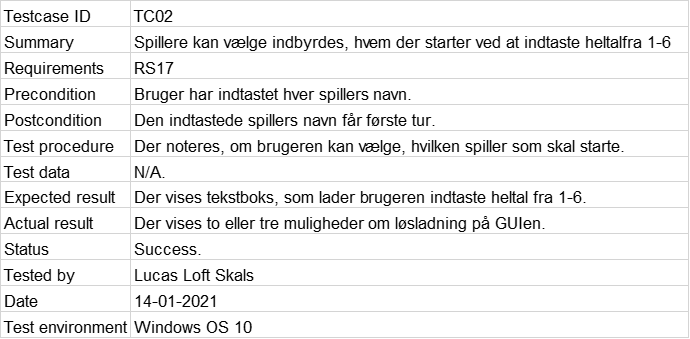
\includegraphics[width=14cm]{Report/figures/Usertests/TC02.png}
    \caption{Tabel over TC02}
    \label{Testcase02}
\end{figure}

I TC03  testes der for, hvorvidt en bruger kan købe grunde i spillet (se Figure \ref{Testcase03}). Dette blev testet ved at starte spillet, hvorefter der noteres, hvorvidt en bruger kan købe grunde, når der landes på et felt. Yderligere hvorvidt GUIen opdateres, så grunden nu tilhører den spiller som købte den. Det endelige resultat af GUIen kan ses i bilagene (se bilag \ref{TC03Bilag}).

\begin{figure}[H] %brug begin{figure} til alle figurer.
    \centering
    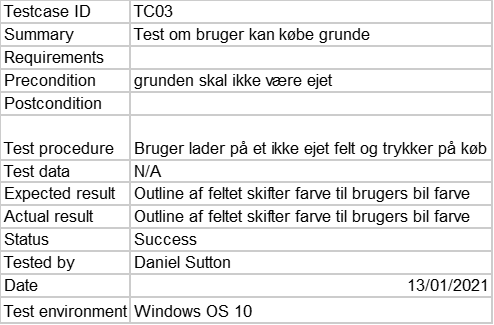
\includegraphics[width=14cm]{Report/figures/Usertests/TC03.png}
    \caption{Tabel over TC03}
    \label{Testcase03}
\end{figure}

\newpage
\subsection{JUnit tests}

Da brugertestene ikke ville være for omfattende, hvis de skulle teste det meste af vores kode, har vi valgt at benytte JUnit tests til, at køre automatiserede tests for det meste af koden der ikke er afhængig af en GUI og et brugerinput.
Nedenunder kan der ses hvor meget code coverage vi har på vores JUnit tests.

\begin{figure}[H] %brug begin{figure} til alle figurer.
    \centering
    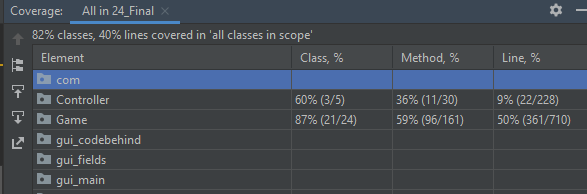
\includegraphics[width=14cm]{Report/figures/Unittests/testcodecoverage.PNG}
    \caption{Oversigt af code coverage på unit tests}
    \label{Testcodecoverage}
\end{figure}

\begin{figure}[H] %brug begin{figure} til alle figurer.
    \centering
    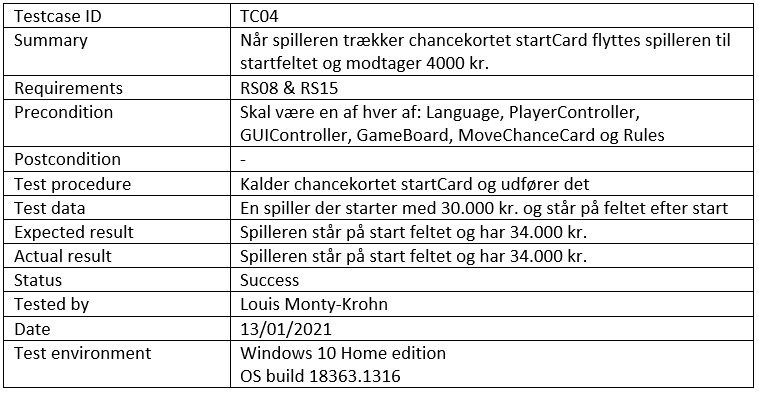
\includegraphics[width=14cm]{Report/figures/Unittests/TC04.PNG}
    \caption{Tabel over TC04}
    \label{Testcase04}
\end{figure}

I TC04 ønsker vi at teste chancekortet startCard's funktion. Dette chancekort skal rykke spilleren der trækker kortet hen til feltet "Start" og dermed modtage 4.000 kr. Dette gør vi ved at lave et spillerobjekt der står på feltet 1, der er feltet efter "Start" der har positionen 0. Herefter bruger vi metoden startCard, og tjekker om spillerens position er 0 og om hans konto er 34.000, da et nyt spillerobjekt starter med en konto på 30.000 kr. Koden kan ses i \ref{TC04Bilag}

\begin{figure}[H] %brug begin{figure} til alle figurer.
    \centering
    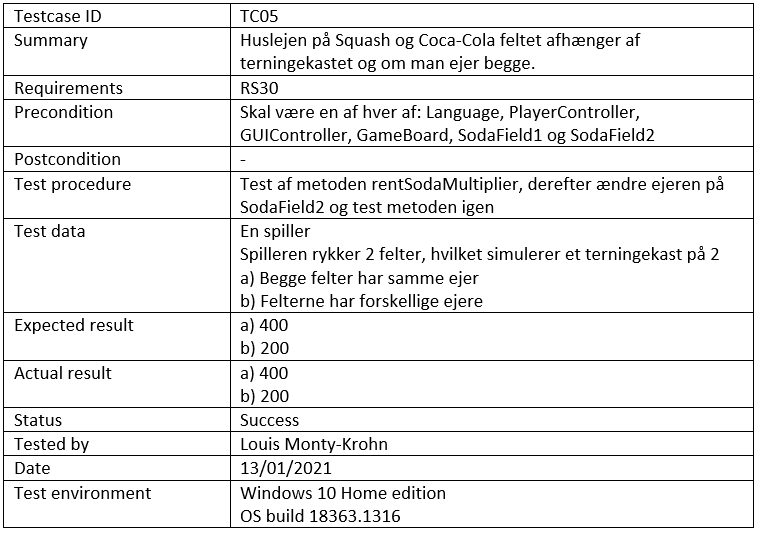
\includegraphics[width=14cm]{Report/figures/Unittests/TC05.PNG}
    \caption{Tabel over TC05}
    \label{Testcase05}
\end{figure}

TC05 tester specifikt, at huslejen bliver regnet korrekt ud på felterne for Squash og Coca-Cola, der er deres egen kategori af felter.
Her skal huslejen regnes ud fra terningkastet. Da vi har en variable numberOfMoves der trækker informationen fra DieControlleren, kan vi bruge denne til at simulere et terningkast. Hvis en anden spiller ejer begge felter bliver huslejen fordoblet.
Så ved at lave et spillerobjekt og to SodaFields kan vi sætte ejeren til en anden værdi end spillerobjektet vi har lavet til testen.
Først simulere vi, at der er slået 2, og tester huslejen hvis begge felter har samme ejer bliver 400. Derefter ændrer vi ejeren af det ene felt, og tester igen om huslejen så bliver 200. Koden kan ses i \ref{TC05Bilag}

\begin{figure}[H] %brug begin{figure} til alle figurer.
    \centering
    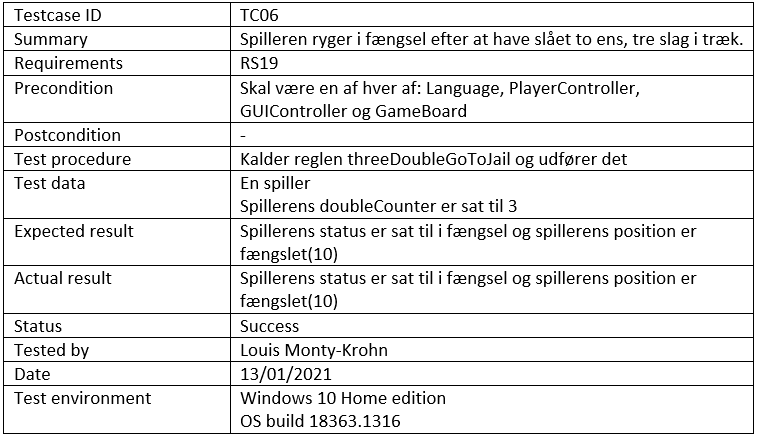
\includegraphics[width=14cm]{Report/figures/Unittests/TC06.PNG}
    \caption{Tabel over TC06}
    \label{Testcase06}
\end{figure}

Vi tester i TC06 om reglen threeDoubleGoToJail virker, altså at man ryger i fængsel efter at have slået to ens, tre slag i træk.
Her laver vi et objekt og ændrer værdien af antal gange spilleren har slået to ens til 3. Derefter bruger vi metoden threeDoubleGoToJail og kigger på spillerens position og status, da begge skal indikere at spilleren er røget i fængsel; inJail = true og playerPosition = 10.
Koden kan ses i \ref{TC06Bilag}


\end{flushleft}